\section{Diego Guadalupe Gomez Hernandez}
\subsection{Definiciones}
\begin{enumerate}
    \item Estudio: Esfuerzo que pone el entendimiento aplicándose a conocer algo o   trabajo empleado en aprender y cultivar una ciencia o arte.
    \item Trabajo: Acción y efecto de trabajar.
    \item Latex: Este es un compositor y compilador de textos que contiene un sistema de composición tipográfica de alta calidad el cual es usado en la publicacion de documentos cientificos en diferentes campo ya que este software es gratis.
    \cite{brys2019tesis}
    \item Github: Es un repositorio  para crear proyectos abiertos de herramientas y aplicaciones teniendo funciones colaborativas ayudando a que puedan trabajar muchas personas en el mismo archivo. 
    \cite{yúbalfernández_2019}
    \item Git: Es un codigo con mantenimiento activo
    \cite{astigarraga2022se}
    \item Funcion: Sirve para descubrir fenomenos de variacion y cambio.
    \item Exactitud: Se define con respecto a su cercania (sesgo), entre mayor cercania implica un buen grado de exactitud.  
    \item Preciso: Es la variacion o dispercion en la cual poca variacion implica un buen grado de precision.
    \item Estudio de movimientos y tiempos: Es el analisis de metodos, materiales, herramientas e instalacion utilizada o que se ah de utilizar en la ejecucion de un trabajo.
    \item Analisis: Distinción y separación de las partes de algo para conocer su composición.
    \cite{RAE2023}
    \item Sistema: Conjunto de reglas o principios sobre una materia racionalmente enlazados entre sí.
    \cite{asale_rae_2023}
    \item Tiempo: Duración de las cosas sujetas a mudanza.
    \item Sistemas de tiempo predeterminado: Conjunto de reglas o metodos para determinar con aticipacion la secuencias de sucesos.
    \item Medicion de tiempos de metodos(MTM): Es un procedimiento que permite el análisis de todo método manual descomponiéndolo en los movimientos básicos requeridos y asignando a cada movimiento un tiempo estándar predeterminado basado en la naturaleza del movimiento y en las condiciones en las que es realizado.
    \item Muestreo: Accion de escoger muestreosque describen de manera exacta las caracteristicas de un conjunto de datos que permitiran deducir y sacar conclusiones del fenomeno a estudiar.
    \item Representativo: Que sirve para representar algo.
    \item Inferir:  Deducir algo o sacarlo como conclusión de otra cosa. Producir un daño físico o moral.
    \cite{asalerae2023}
    \item Alcanzar: Movimiento realizado con la mano vacia.
    \cite{asale_rae_2023}
    \item Mover: Movimiento con un objeto en la mano.
    \item Muestreo de trabajo: Herramienta para disminuir el costo que se presenta en el estudio continuo del tiempo.
    \item Estudio de tiempos convencional: Es una muestra continua de n ciclos (Suponiendo que la distribución estadística es normal).
    \item Estudio de tiempos no convencional: Es una muestra discreta (Suponiendo que la distribución estadística es binomial).
\end{enumerate}
\subsection{Materiales}
\begin{table}[H]
    \centering
    \begin{tabular}{|c|c|c|}
    \hline
    \multicolumn{3}{|c|}{MATERIALES} \\
    \hline 
    NOMBRE & CANTIDAD & PLANO \\
    \hline 
    ESP32-C6 & 1 & 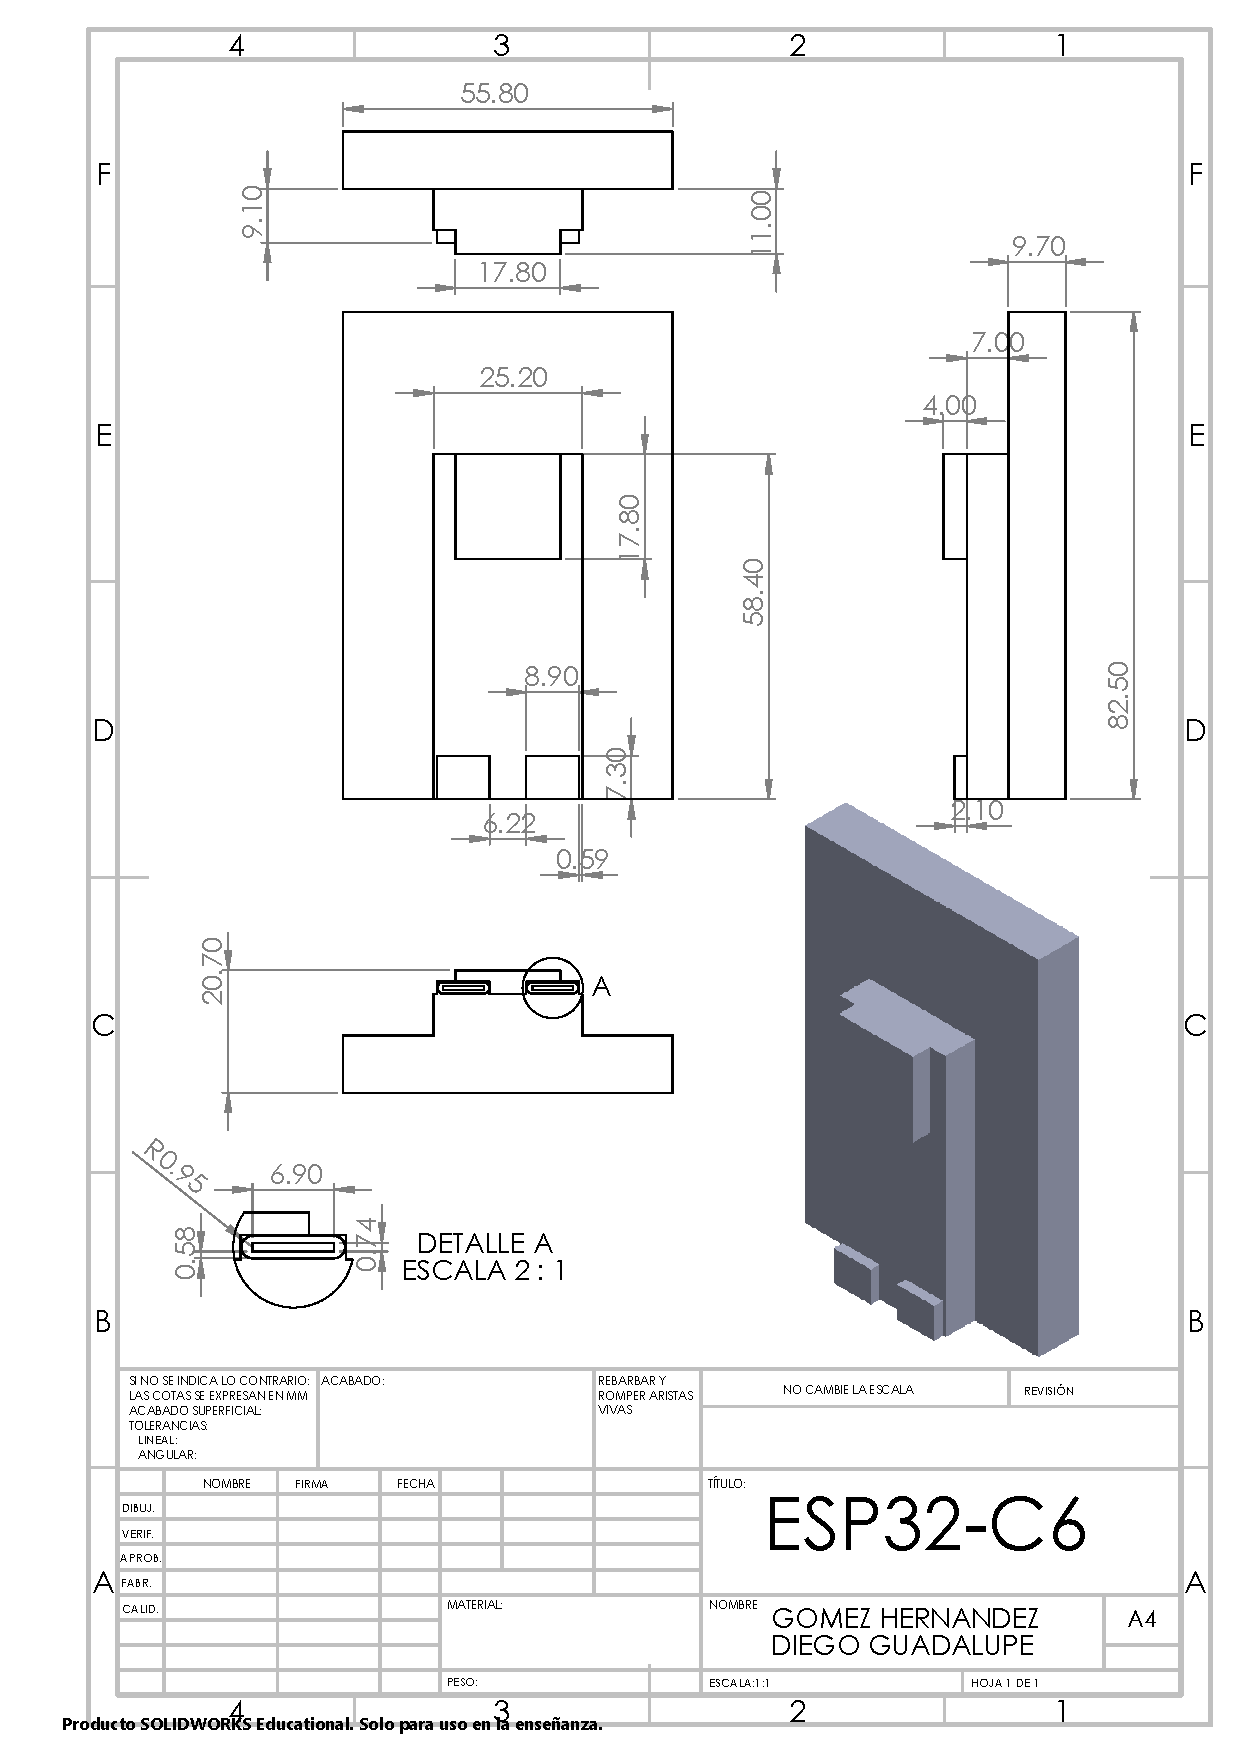
\includegraphics[width=.135\textwidth]{13/img/DIBUJO ESP.pdf} \\
    \hline 
    LCD 16x2 & 1 & 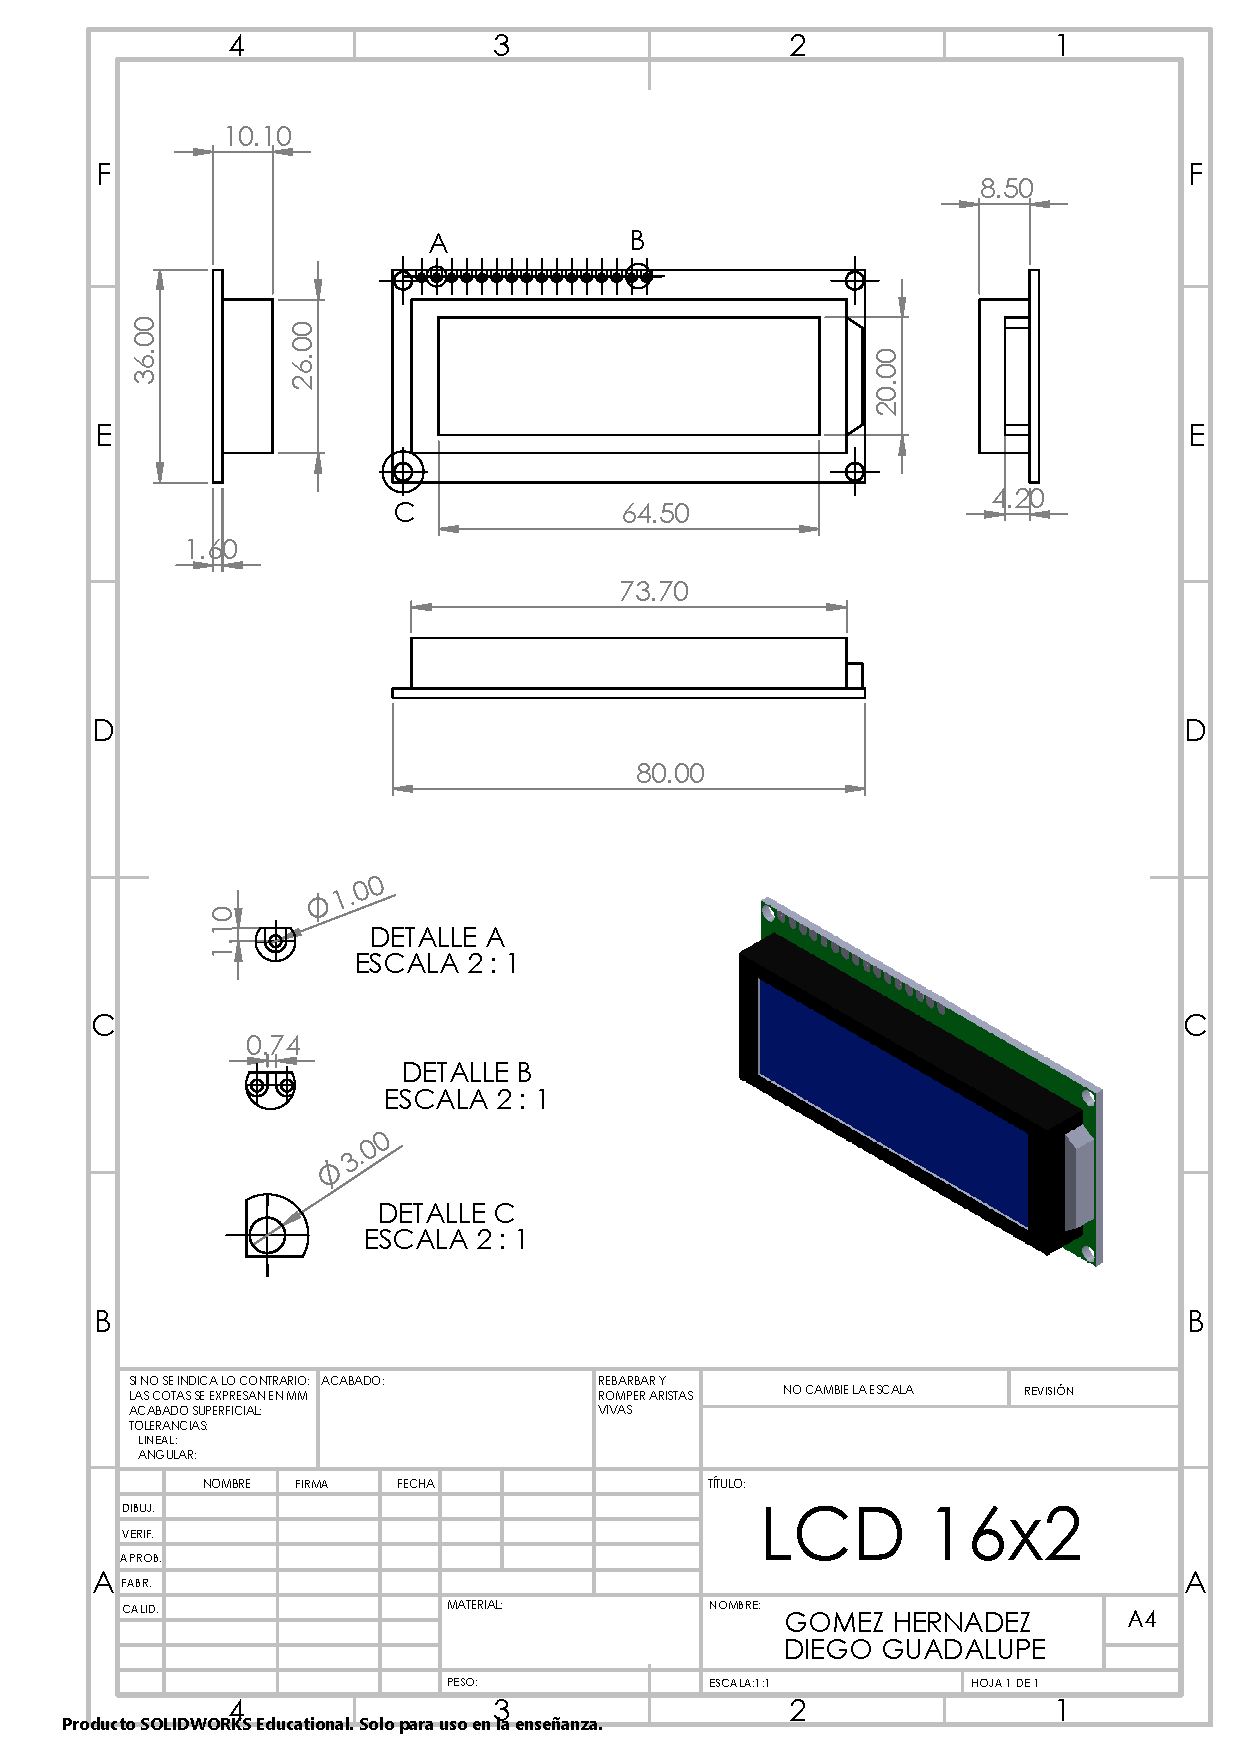
\includegraphics[width=.135\textwidth]{13/img/DIBUJO lcd.pdf}  \\
    \hline
    Potenciometro 1K ohm & 1 &  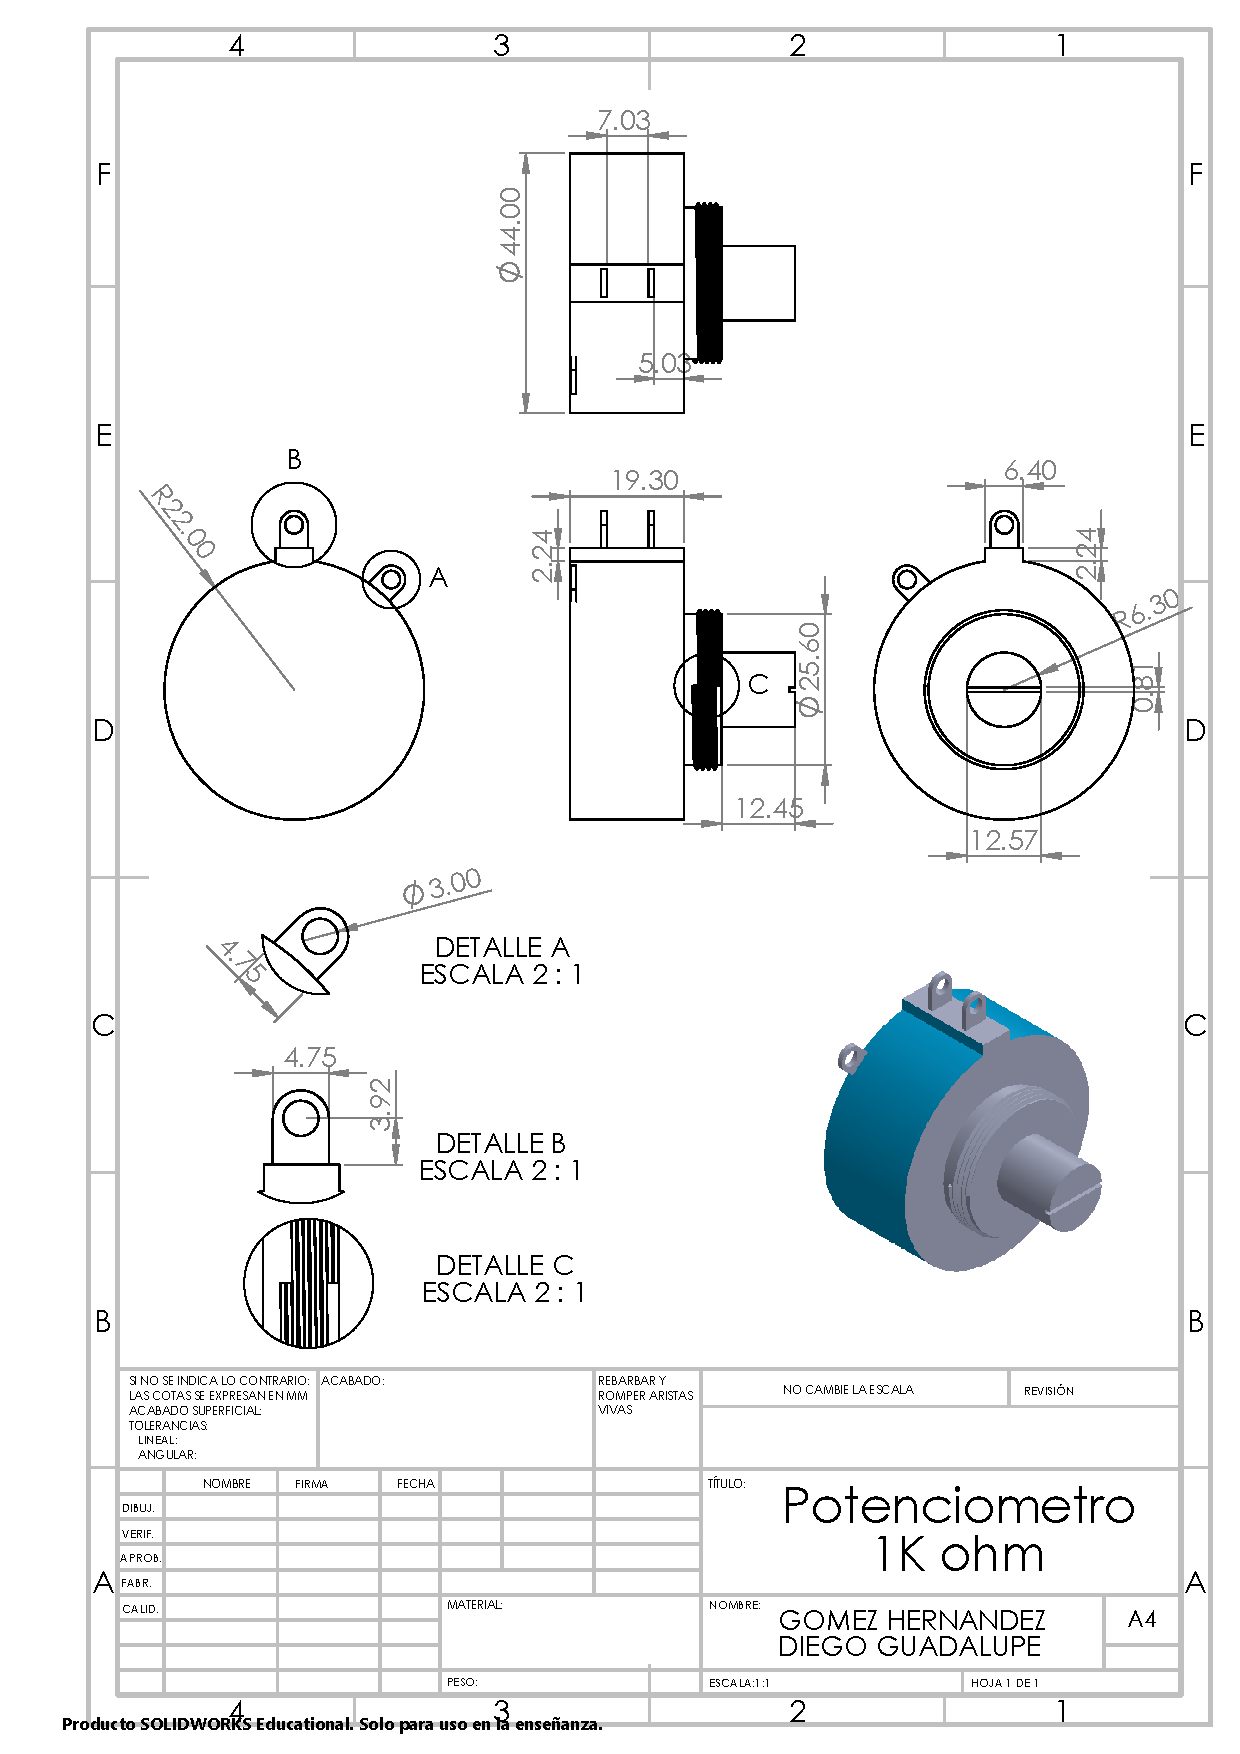
\includegraphics [width=.135\textwidth]{13/img/DIBUJO potenciometro.pdf} \\
    \hline
    Resistencias & 2 & 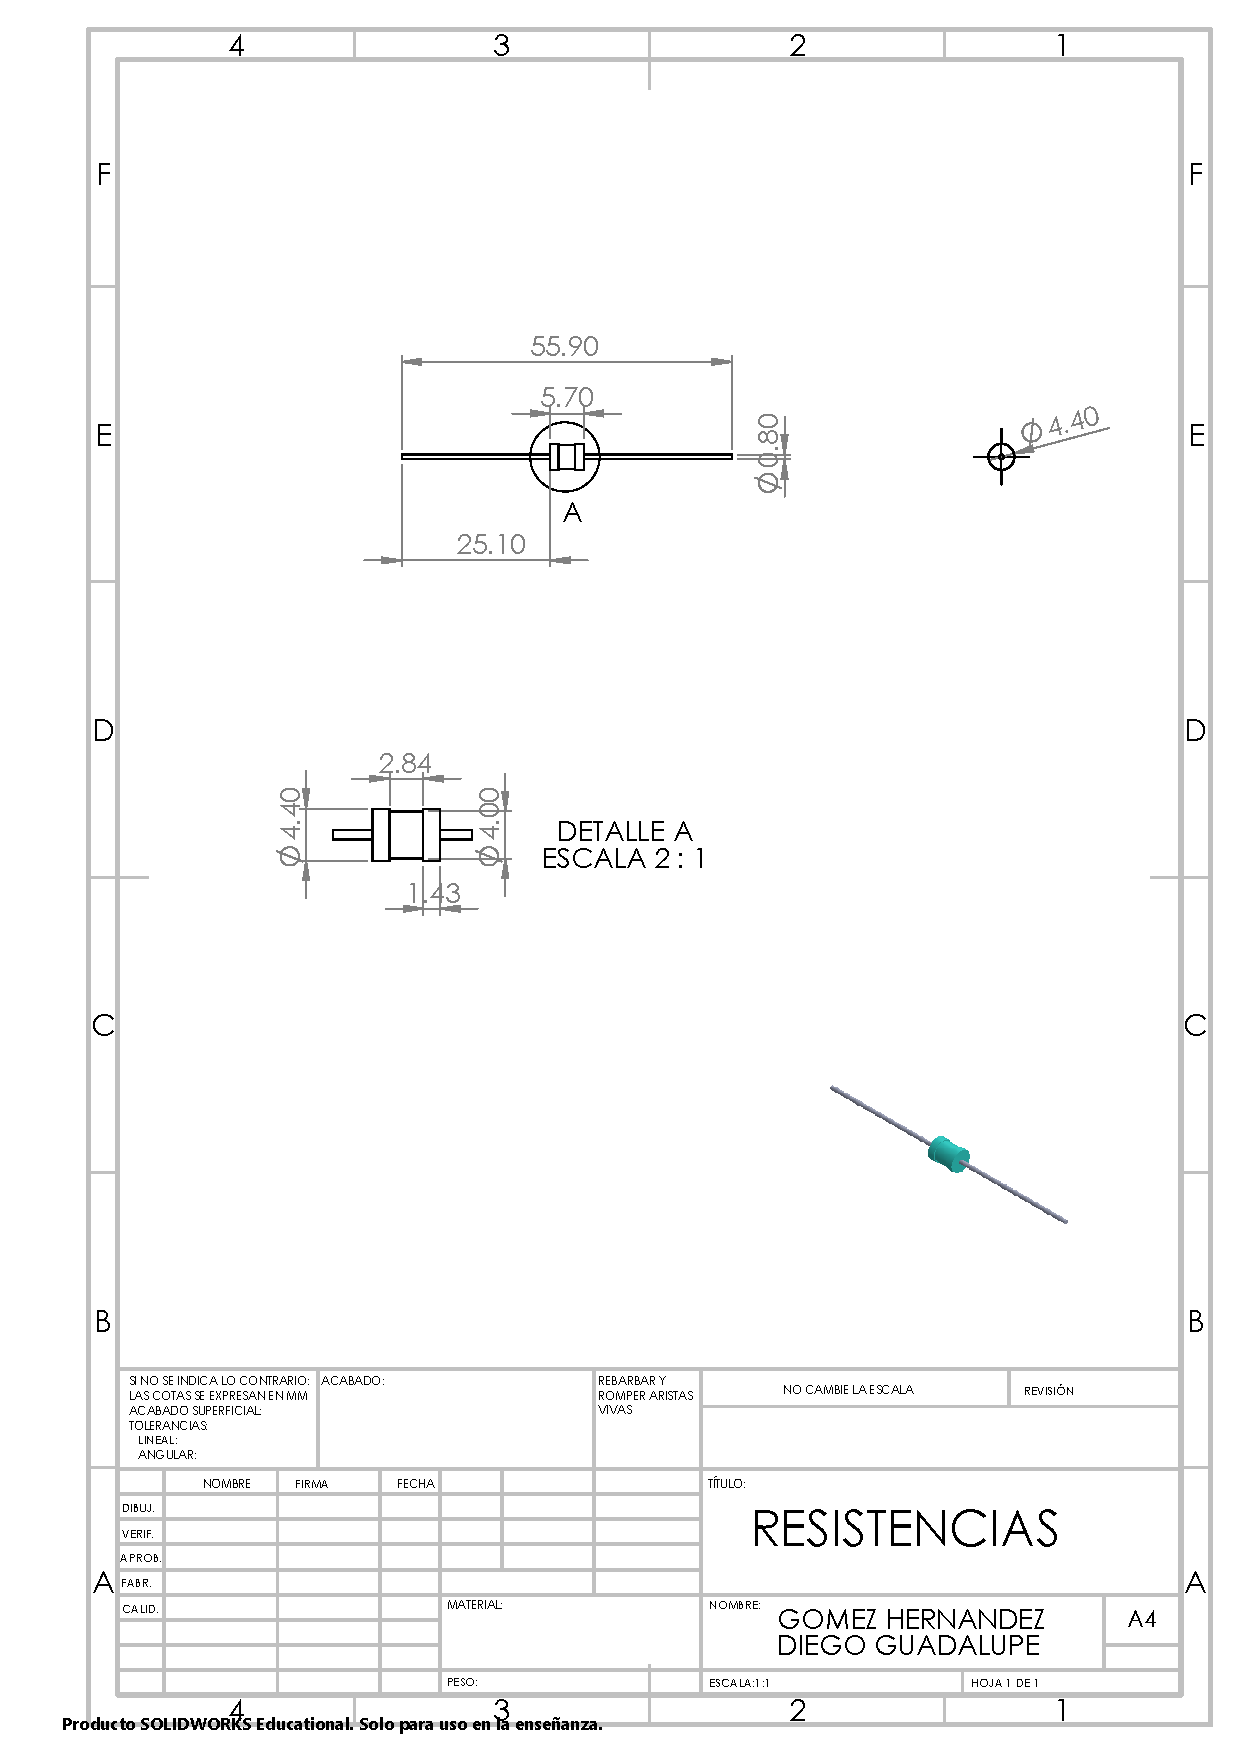
\includegraphics[width=.135\textwidth]{13/img/DIBUJO resistencia.pdf}  \\
    \hline
    Cable m-m & 6 & 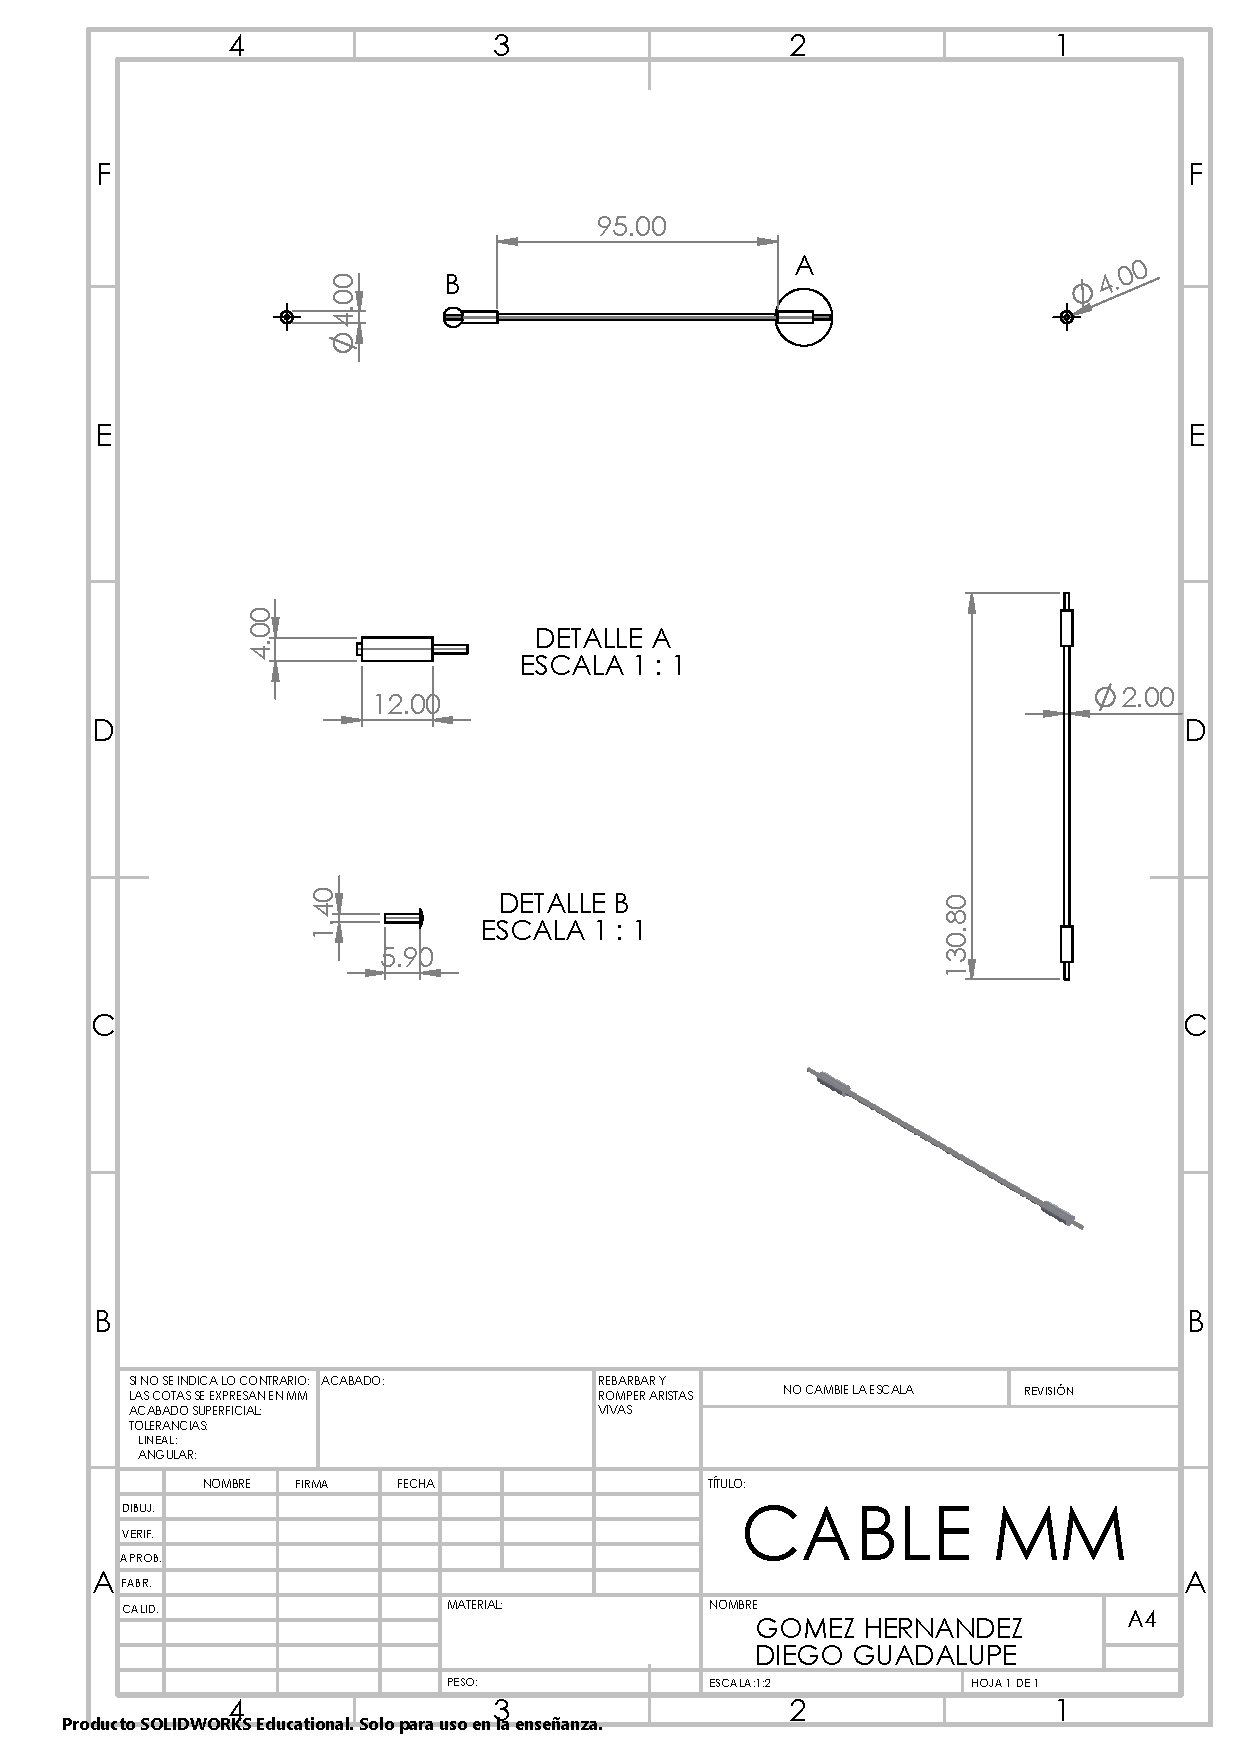
\includegraphics[width=.135\textwidth]{13/img/DIBUJO mm.pdf}  \\
    \hline
    Cable m-h & 4 & 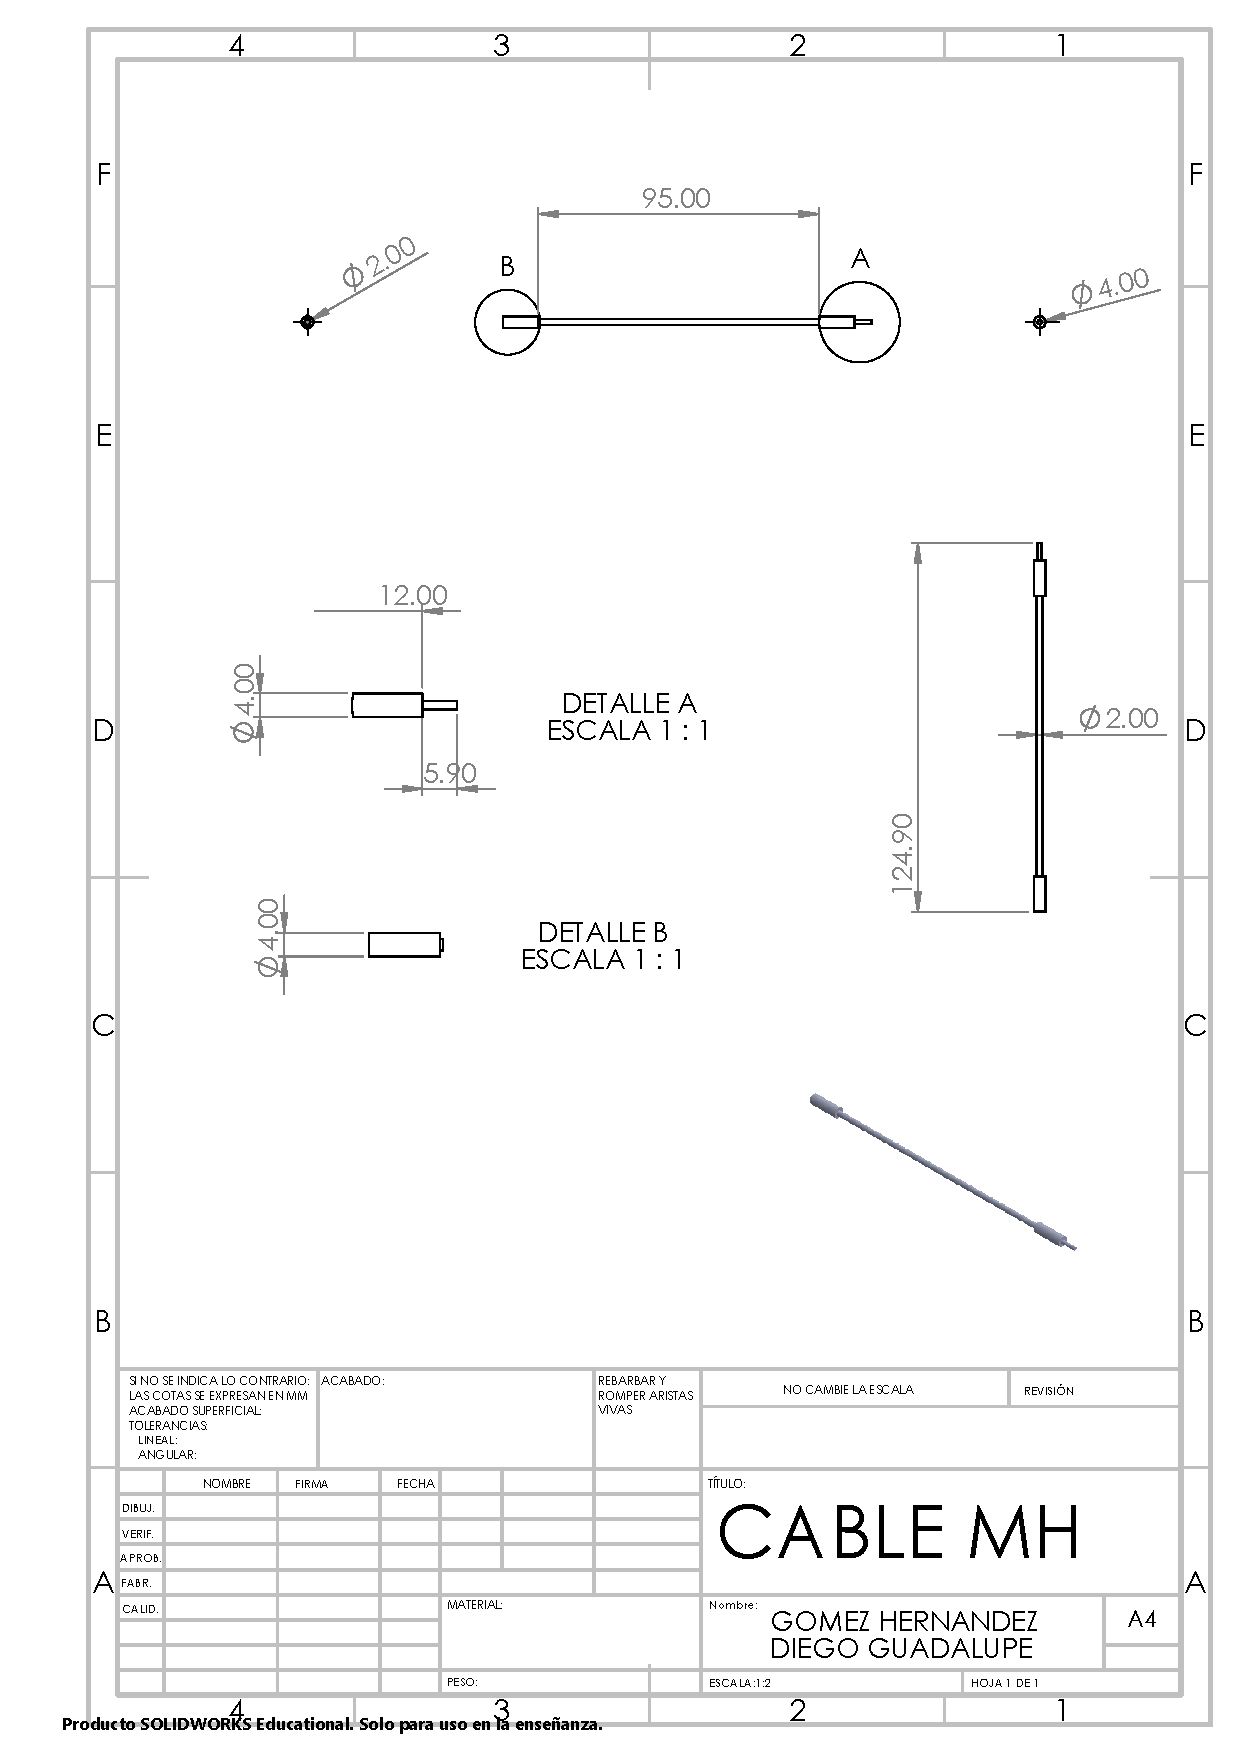
\includegraphics[width=.135\textwidth]{13/img/DIBUJO mh.pdf}  \\
    \hline
    \end{tabular}
    \caption{MATERIALES}
    \label{tab:my_label}
\end{table}
\subsection{Desarrollo}

\bibliographystyle{apalike}
\bibliography{13/referencias}
